\section{Erweiterte Partitionierung: Partitionen anlegen}
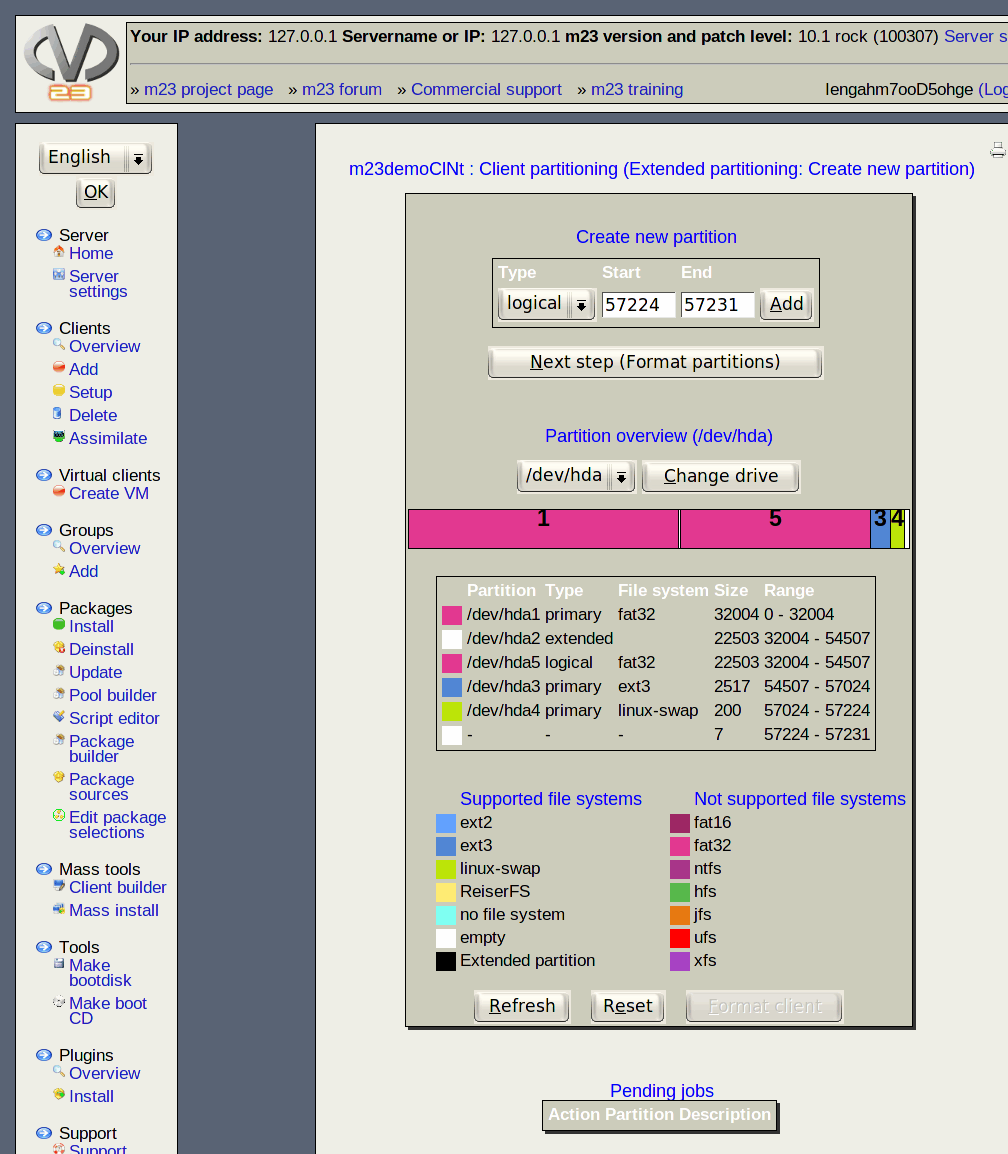
\includegraphics[scale=0.4]{/mdk/doc/manual/screenshots/de/fdisk-extended1.png} \\
\begin{itemize}
\item Nun k�nnen Sie neue Partitionen anlegen. W�hlen Sie aus, ob Sie eine prim�re (primary), erweiterte (extended) oder logische (logical) Partition erstellen m�chten.\\
W�hlen Sie den Typ und den Start- und End-Punkt der Partition und klicken Sie danach auf \textit{"Hinzuf�gen"}. Unter Typ k�nnen Sie nur Partitionstypen ausw�hlen, die Sie tats�chlich anlegen k�nnen. Zu den Bedingungen zum Anlegen der Partitionstypen finden Sie unten einen Hinweis.\\
\item Unter \textit{"Partitions-�berblick"} finden Sie freie Bereiche (wei� gekennzeichnet), in denen Sie neue Partitionen anlegen k�nnen. Als Anhaltspunkt f�r die Start- und End-Werte Ihrer neuen Partitionen beachten Sie bitte die Werte unter \textit{"Bereich"}.\\
\item Sollte nicht gen�gend freier Platz vorhanden sein, um die von Ihnen gew�nschten Partitionen anzulegen, so klicken Sie wiederholt auf den \textit{"Zur�ck"}-Button Ihres Browsers, bis Sie zur \textit{"Partitionen l�schen"}-Seite gelangen.\\
\item Haben Sie alle ben�tigten Partitionen angelegt, dann klicken Sie auf \textit{""}.\\
\end{itemize}
\subsection{Information: Partitionstypen}
\begin{itemize}
 \item \textbf{prim�r:} Sie k�nnen maximal 4 prim�re Partitionen anlegen.\\
 \item \textbf{erweitert:} Eine erweiterte Partition z�hlt ebenfalls zu den prim�ren Partitionen. Es kann maximal eine erweiterte Partition angelegt werden. Innerhalb einer erweiterten Partition k�nnen Sie logische Partitionen anlegen, falls Ihnen 4 prim�re nicht reichen sollten.\\
 \item \textbf{logisch:} Logische Partitionen k�nnen nur im Speicherplatz einer erweiterten Partition angelegt werden. Die Anzahl der logischen Partitionen ist nicht beschr�nkt.\\
\end{itemize}
